% Intended LaTeX compiler: pdflatex
\documentclass[10pt,a4paper,UTF8]{article}
\usepackage{zclorg}
\date{}
\title{内积与范数}
\hypersetup{
 pdfauthor={},
 pdftitle={内积与范数},
 pdfkeywords={},
 pdfsubject={},
 pdfcreator={Emacs 25.0.50.1 (Org mode 9.0.5)},
 pdflang={English}}
\begin{document}

\maketitle
\tableofcontents
\titlepic{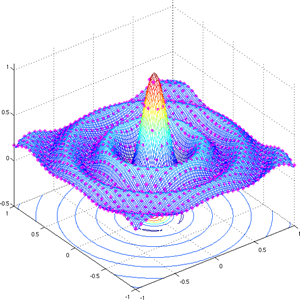
\includegraphics[scale=0.25]{../../img/sinc.PNG}}


\section{内积}
\label{sec:orgbf74ed3}


\begin{definition}
\(x=(x_{1},\ldots ,x_{n}) \in \mathbf{R}^{n}\)的范数为:
\begin{equation}
\label{eq:1}
||x|| = \sqrt{x_1^2 + \ldots + x_n^2}
\end{equation}
\end{definition}
范数在\(\mathbf{R}^{n}\)上不是线性的,为了把线性引入讨论,定义点积:

\begin{definition}
对于\(x,y\in \mathbf{R}^{n}\),\(x\)和\(y\)的点积\(x\cdot y\)定义为:
\begin{equation}
\label{eq:2}
x\cdot y = x_{1}y_{1} + \ldots x_{n}y_{n}
\end{equation}
其中\(x = (x_{1},\ldots ,x_{n})\),\(y = (y_{1},\ldots ,y_{n})\)
\end{definition}
注意\(\mathbf{R}^{n}\)中两个向量的点积是一个数。对所有的\(x\in \mathbf{R}^{n}\),均有\(x\cdot x = ||x||^{2}\),\(\mathbf{R}^{n}\)上的点积具有如下性质:
\begin{enumerate}
\item 对所有\(x\in \mathbf{R}^{n}\),均有\(x\cdot x \geq 0\)
\item \(x\cdot x = 0\),当且仅当\(x = 0\)
\item 对于固定的\(y\in \mathbf{R}^{n}\),\(\mathbf{R}^{n}\)到\(R\)的将\(x\in \mathbf{R}^{n}\)变为\(x\cdot y\)的映射是线性的。
\item 对所有\(x,y\in \mathbf{R}^{n}\),有\(x\cdot y = y\cdot x\)
\end{enumerate}

内积是点积的推广。定义内积就是抽象化点积的过程:
\begin{definition}
\(V\)上的内积就是一个函数,把\(V\)中的元素的每个有序对\(u,v\)都映成一个数\(\langle u,v \rangle\) 并且具有以下性质:
\begin{enumerate}
\item 对所有的\(v\in V\),有\(\langle v,v \rangle \geq 0\)
\item \(\langle v,v \rangle =  0\),当且仅当\(v=0\)
\item 对所有\(u,v,w\in V\),均有\(\langle u+v,w \rangle = \langle u,w \rangle + \langle v,w \rangle\)
\item 对所有\(\lambda\in \mathbf{F}\)和所有\(u,v\in V\),有\(\langle \lambda u,v \rangle = \lambda \langle u,v \rangle\)
\item 对所有\(u,v\in V\),有\(\langle u,v \rangle = \overline{ \langle v,u \rangle }\)
\end{enumerate}
\end{definition}

\begin{instance}
\(\mathbf{F}^{n}\)上的欧几里得内积定义为:
\begin{equation}
\label{eq:3}
\langle (w_{1},\ldots ,w_{n}),(z_{1},\ldots ,z_{n}) \rangle = w_{1}\bar{z_{1}} + \ldots + w_{n}\bar{z_{n}}
\end{equation}
\end{instance}

\begin{instance}
若\(c_{1},\ldots ,c_{n}\)均为正数,则可以定义\(\mathbf{F}^{n}\)上的内积:
\begin{equation}
\label{eq:4}
\langle (w_{1},\ldots ,w_{n}),(z_{1},\ldots ,z_{n}) \rangle = c_{1}w_{1}\bar{z_{1}} + \ldots + c_{n}w_{n}\bar{z_{n}}
\end{equation}
\end{instance}

\begin{instance}
在定义区间\([-1,1]\)上的实值连续函数构成的向量空间上可定义内积如下:
\begin{equation}
\label{eq:5}
\langle f,g \rangle = \int_{-1}^{1}f(x)g(x) \mathrm{d} x
\end{equation}
\end{instance}
\begin{instance}
在\(\mathcal{P}(\mathbf{R})\)上可定义内积如下:
\begin{equation}
\label{eq:6}
\langle p,q \rangle = \int_{0}^{\infty}p(x)q(x)e^{-x} \mathrm{d}x
\end{equation}
\end{instance}
\begin{definition}
内积空间就是带有内积的向量空间 \(V\)
\end{definition}
内积空间最重要的例子是\(\mathbf{F}^{n}\),当我们说\(\mathbf{F}^{n}\)是内积空间的时候,我们总假设采用的是欧几里得内积。

\begin{theorem}
\begin{enumerate}
\item 对每个确定的\(u\in V\),将\(v\)变为\(v,u\)的函数是\(V\)到\(\mathbf{F}\)的线性映射。
\item 对每个\(u\in V\),均有\(\langle 0,u \rangle  = 0\)
\item 对每个\(u\in V\),均有\(\langle u,0 \rangle  = 0\)
\item 对所有\(u,v,w\in V\)均有\(\langle u,v+w \rangle = \langle u,v \rangle  + \langle u,w \rangle\)
\item 对所有\(\lambda\in \mathbf{F}\)和所有\(u,v\in V\)均有\(\langle u,\lambda v \rangle = \bar{\lambda} \langle u,v \rangle\)
\end{enumerate}
\end{theorem}
\section{范数}
\label{sec:org2b0c3d3}


\begin{definition}
对于\(v\in V\),\(v\)的范数\(\|v\| = \sqrt{\langle v,v \rangle }\)
\end{definition}

\begin{instance}
若\((z_{1},\ldots ,z_{n}) \in \mathbf{F}^{n}\),则:
\begin{equation}
\label{eq:7}
\| (z_{1},\ldots ,z_{n}) \| = \sqrt{ |z_{1}|^{2} + \ldots + |z_{n}|^{2}}
\end{equation}
\end{instance}

\begin{instance}
在\([-1,1]\)上的实值连续函数构成的向量空间中有:
\begin{equation}
\label{eq:8}
\| f \| = \sqrt{\int_{-1}^{1} (f(x))^{2} \mathrm{d}x }
\end{equation}
\end{instance}
范数的基本性质:
\begin{theorem}
设\(v\in V\)
\begin{enumerate}
\item \(\| v\| = 0\) 当且仅当\(v=0\)
\item 对所有\(\lambda\in \mathbf{F}\)均有\(\| \lambda v\| = |\lambda| \|v\|\)
\end{enumerate}
\end{theorem}
通常,处理范数的平方要比直接处理范数更容易。

\begin{definition}
两个向量\(u,v\in V\)是正交的,如果\(\langle u,v \rangle  = 0\)
\end{definition}

若\(u,v\)是\(\mathbf{R}^{2}\)中的非零向量,则:
\begin{equation}
\label{eq:9}
\langle u,v \rangle = \| u \| \| v\|\cos \theta
\end{equation}

其中\(\theta\)是\(u\)和\(v\)的夹角,显然在平面几何的意义下,正交意味着垂直。

\begin{theorem}
\begin{enumerate}
\item \(0\)正交与\(V\)中的任意向量。
\item \(0\)是\(V\)中唯一一个与自身正交的向量。
\end{enumerate}
\end{theorem}

\begin{theorem}
设\(u\)和\(v\)是\(V\)中的正交向量,则\(\| u+v \|^{2} = \| u \|^{2} + \| v \|^{2}\)
\end{theorem}

\begin{proof}
\begin{eqnarray}
\label{eq:10}
\| u+v \|^{2} &=& \langle (u+v),(u+v) \rangle  \\
&=& \langle u,u \rangle  + \langle u,v \rangle  + \langle v,u \rangle + \langle v,v \rangle \\
&=& \langle u,u \rangle  + \langle v,v \rangle \\
&=& \| u \|^{2} + \| v \|^{2}
\end{eqnarray}
\end{proof}

设\(u,v\in V\),且\(v\neq 0\),我们想把\(u\)写成\(v\)的标量倍加上一个正交与\(v\)的向量\(w\)。如图\ref{fig:orge90be60}所示:
\begin{figure}[htbp]
\centering
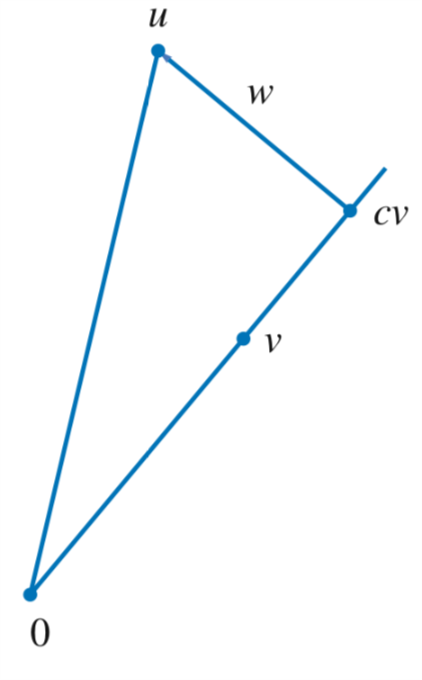
\includegraphics[width=0.5\textwidth]{../../img/math_ladr/20170514orthogonalDecomposition.png}
\caption{\label{fig:orge90be60}
正交分解}
\end{figure}

为了揭示如何将\(u\)写成\(v\)的标量倍加上一个正交于\(v\)的向量,令\(c\in \mathbf{F}\)表示一个标量,则:
\[u = cv + (u-cv)\]
因此需要选取\(c\)使得\(v\)正交于\(u-cv\),也就是说我们希望:
\[0 = \langle u-cv,v \rangle  = \langle u,v \rangle - c \| v \|^{2}  \]
上式表明\(c\)应该是\[\langle u,v \rangle / \| v \|^{2}  \] 从而
\[ u =  \frac{\langle u,v \rangle  }{\| v \|^{2} }v + (u - \frac{\langle u,v \rangle  }{\| v \|^{2} } v) \]
上式把\(u\)写成了\(v\)的标量倍加上一个正交于\(v\)的向量。
\begin{theorem}
设\(u,v\in V\)且\(v\neq 0\),令\(c = \frac{\langle u,v \rangle  }{\| v \|^{2} }, w = u - \frac{\langle u,v \rangle  }{\| v \|^{2} } v\)则\(\langle w,v \rangle = 0\),且\(u = cv + w\)
\end{theorem}

\begin{theorem}
设\(u,v\in V\),则 \(| \langle u,v \rangle  | \leq \| u \| \| v \|\),等号成立当且仅当\(u,v\)之间存在标量倍的关系。
\end{theorem}

\begin{proof}
我们把\(u\)分解为:
\[u = w + \frac{\langle u,v \rangle  }{\| v \|^{2} } v\]
其中\(w\)正交与\(v\),根据勾股定理,我们有:
\begin{eqnarray}
\label{eq:11}
\| u \|^{2} &=& \bigg\| \frac{\langle u,v \rangle  }{\| v \|^{2} } v \bigg\|^{2}  + \| w \|^{2} \\
&=& \frac{ \|\langle u,v \rangle \|^{2}  }{\| v \|^{2} }  + \| w \|^{2} \\
&\geq & \frac{ \|\langle u,v \rangle \|^{2}  }{\| v \|^{2} }
\end{eqnarray}
\end{proof}
柯西施瓦茨不等式的例子
\begin{instance}
若\(x_{1},\ldots ,x_{n},y_{1},\ldots ,y_{n}\in \mathbf{R}\),则:
\begin{equation}
\label{eq:12}
|x_1y_1 + \ldots x_ny_n|^2 \leq (x_1^2 + \ldots x_n^2)(y_1^2 + \ldots + y_n^2)
\end{equation}
\end{instance}
\begin{instance}
若\(f,g\)均为\([-1,1]\)上的实值连续函数,则:
\begin{equation}
\label{eq:13}
\bigg\vert \int_{-1}^{1}f(x)g(x)dx \bigg\vert^{2} \leq \bigg(\int_{-1}^{1} (f(x))^{2}dx\bigg) \bigg(\int_{-1}^{-1} (g(x))^{2}dx\bigg)
\end{equation}
\end{instance}

\begin{theorem}
设\(u,v\in V\),则\(\| u + v \| \leq \| u \| +  \| v \|\),等号成立当且仅当\(u,v\)之一是另一个的标量倍。
\end{theorem}
\begin{proof}
\begin{eqnarray}
\label{eq:14}
\| u+v \|^{2} &=& \langle u+v,u+v \rangle  \\
&=& \langle u,u \rangle  + \langle u,v \rangle  + \langle v,u \rangle  + \langle v,v \rangle  \\
&\leq& \| u \|^{2} + \| v \|^{2} + 2 \| u \| \| v \| \\
&=& ( \| u \| + \| v \| )^{2}
\end{eqnarray}
所以 \(\| u + v \| \leq \| u \| + \| v \|\)
\end{proof}

\begin{theorem}
设\(u,v\in V\),则\(\| u + v \|^{2} + \| u-v \|^{2} = 2( \| u \|^{2} + \| v \|^{2})\)
\end{theorem}
\begin{proof}
\begin{eqnarray}
\label{eq:15}
\| u+v \|^{2} + \| u-v \|^{2} &=& \langle u + v,u+v \rangle   + \langle u-v,u-v \rangle  \\
&=& \langle u,u \rangle  + \langle u,v \rangle + \langle v,u \rangle + \langle v,v \rangle \\
&+& \langle u,u \rangle + \langle u,-v \rangle + \langle -v,u \rangle + \langle -v,-v \rangle \\
&=& 2 \langle u,u \rangle  + 2 \langle v,v \rangle \\
&=& 2( \| u \|^{2} + \| v \|^{2} )
\end{eqnarray}
\end{proof}
\end{document}
